\documentclass[1p]{elsarticle_modified}
%\bibliographystyle{elsarticle-num}

%\usepackage[colorlinks]{hyperref}
%\usepackage{abbrmath_seonhwa} %\Abb, \Ascr, \Acal ,\Abf, \Afrak
\usepackage{amsfonts}
\usepackage{amssymb}
\usepackage{amsmath}
\usepackage{amsthm}
\usepackage{scalefnt}
\usepackage{amsbsy}
\usepackage{kotex}
\usepackage{caption}
\usepackage{subfig}
\usepackage{color}
\usepackage{graphicx}
\usepackage{xcolor} %% white, black, red, green, blue, cyan, magenta, yellow
\usepackage{float}
\usepackage{setspace}
\usepackage{hyperref}

\usepackage{tikz}
\usetikzlibrary{arrows}

\usepackage{multirow}
\usepackage{array} % fixed length table
\usepackage{hhline}

%%%%%%%%%%%%%%%%%%%%%
\makeatletter
\renewcommand*\env@matrix[1][\arraystretch]{%
	\edef\arraystretch{#1}%
	\hskip -\arraycolsep
	\let\@ifnextchar\new@ifnextchar
	\array{*\c@MaxMatrixCols c}}
\makeatother %https://tex.stackexchange.com/questions/14071/how-can-i-increase-the-line-spacing-in-a-matrix
%%%%%%%%%%%%%%%

\usepackage[normalem]{ulem}

\newcommand{\msout}[1]{\ifmmode\text{\sout{\ensuremath{#1}}}\else\sout{#1}\fi}
%SOURCE: \msout is \stkout macro in https://tex.stackexchange.com/questions/20609/strikeout-in-math-mode

\newcommand{\cancel}[1]{
	\ifmmode
	{\color{red}\msout{#1}}
	\else
	{\color{red}\sout{#1}}
	\fi
}

\newcommand{\add}[1]{
	{\color{blue}\uwave{#1}}
}

\newcommand{\replace}[2]{
	\ifmmode
	{\color{red}\msout{#1}}{\color{blue}\uwave{#2}}
	\else
	{\color{red}\sout{#1}}{\color{blue}\uwave{#2}}
	\fi
}

\newcommand{\Sol}{\mathcal{S}} %segment
\newcommand{\D}{D} %diagram
\newcommand{\A}{\mathcal{A}} %arc


%%%%%%%%%%%%%%%%%%%%%%%%%%%%%5 test

\def\sl{\operatorname{\textup{SL}}(2,\Cbb)}
\def\psl{\operatorname{\textup{PSL}}(2,\Cbb)}
\def\quan{\mkern 1mu \triangleright \mkern 1mu}

\theoremstyle{definition}
\newtheorem{thm}{Theorem}[section]
\newtheorem{prop}[thm]{Proposition}
\newtheorem{lem}[thm]{Lemma}
\newtheorem{ques}[thm]{Question}
\newtheorem{cor}[thm]{Corollary}
\newtheorem{defn}[thm]{Definition}
\newtheorem{exam}[thm]{Example}
\newtheorem{rmk}[thm]{Remark}
\newtheorem{alg}[thm]{Algorithm}

\newcommand{\I}{\sqrt{-1}}
\begin{document}

%\begin{frontmatter}
%
%\title{Boundary parabolic representations of knots up to 8 crossings}
%
%%% Group authors per affiliation:
%\author{Yunhi Cho} 
%\address{Department of Mathematics, University of Seoul, Seoul, Korea}
%\ead{yhcho@uos.ac.kr}
%
%
%\author{Seonhwa Kim} %\fnref{s_kim}}
%\address{Center for Geometry and Physics, Institute for Basic Science, Pohang, 37673, Korea}
%\ead{ryeona17@ibs.re.kr}
%
%\author{Hyuk Kim}
%\address{Department of Mathematical Sciences, Seoul National University, Seoul 08826, Korea}
%\ead{hyukkim@snu.ac.kr}
%
%\author{Seokbeom Yoon}
%\address{Department of Mathematical Sciences, Seoul National University, Seoul, 08826,  Korea}
%\ead{sbyoon15@snu.ac.kr}
%
%\begin{abstract}
%We find all boundary parabolic representation of knots up to 8 crossings.
%
%\end{abstract}
%\begin{keyword}
%    \MSC[2010] 57M25 
%\end{keyword}
%
%\end{frontmatter}

%\linenumbers
%\tableofcontents
%
\newcommand\colored[1]{\textcolor{white}{\rule[-0.35ex]{0.8em}{1.4ex}}\kern-0.8em\color{red} #1}%
%\newcommand\colored[1]{\textcolor{white}{ #1}\kern-2.17ex	\textcolor{white}{ #1}\kern-1.81ex	\textcolor{white}{ #1}\kern-2.15ex\color{red}#1	}

{\Large $\underline{12n_{0429}~(K12n_{0429})}$}

\setlength{\tabcolsep}{10pt}
\renewcommand{\arraystretch}{1.6}
\vspace{1cm}\begin{tabular}{m{100pt}>{\centering\arraybackslash}m{274pt}}
\multirow{5}{120pt}{
	\centering
	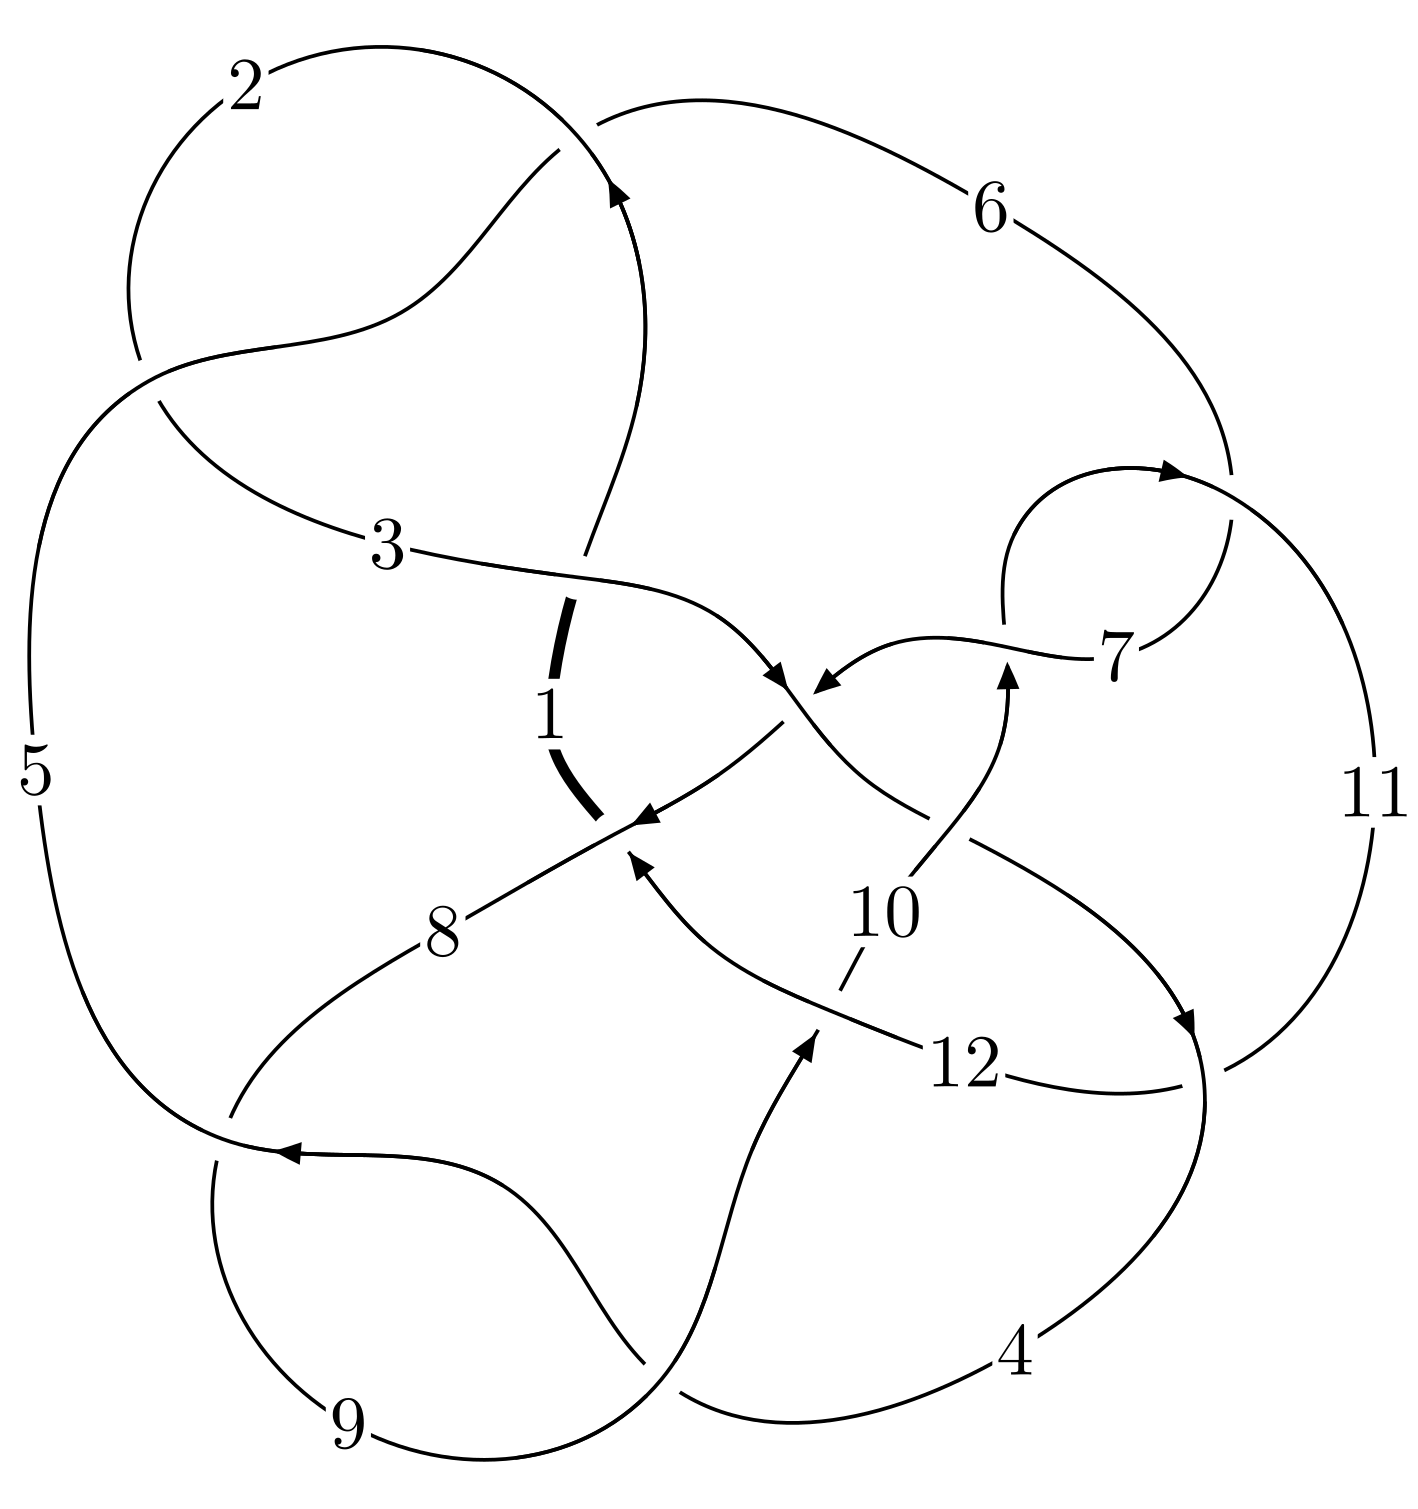
\includegraphics[width=112pt]{../../../GIT/diagram.site/Diagrams/png/2518_12n_0429.png}\\
\ \ \ A knot diagram\footnotemark}&
\allowdisplaybreaks
\textbf{Linearized knot diagam} \\
\cline{2-2}
 &
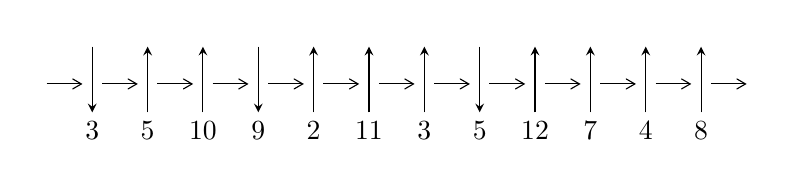
\begin{tikzpicture}[x=20pt, y=17pt]
	% nodes
	\node (C0) at (0, 0) {};
	\node (C1) at (1, 0) {};
	\node (C1U) at (1, +1) {};
	\node (C1D) at (1, -1) {3};

	\node (C2) at (2, 0) {};
	\node (C2U) at (2, +1) {};
	\node (C2D) at (2, -1) {5};

	\node (C3) at (3, 0) {};
	\node (C3U) at (3, +1) {};
	\node (C3D) at (3, -1) {10};

	\node (C4) at (4, 0) {};
	\node (C4U) at (4, +1) {};
	\node (C4D) at (4, -1) {9};

	\node (C5) at (5, 0) {};
	\node (C5U) at (5, +1) {};
	\node (C5D) at (5, -1) {2};

	\node (C6) at (6, 0) {};
	\node (C6U) at (6, +1) {};
	\node (C6D) at (6, -1) {11};

	\node (C7) at (7, 0) {};
	\node (C7U) at (7, +1) {};
	\node (C7D) at (7, -1) {3};

	\node (C8) at (8, 0) {};
	\node (C8U) at (8, +1) {};
	\node (C8D) at (8, -1) {5};

	\node (C9) at (9, 0) {};
	\node (C9U) at (9, +1) {};
	\node (C9D) at (9, -1) {12};

	\node (C10) at (10, 0) {};
	\node (C10U) at (10, +1) {};
	\node (C10D) at (10, -1) {7};

	\node (C11) at (11, 0) {};
	\node (C11U) at (11, +1) {};
	\node (C11D) at (11, -1) {4};

	\node (C12) at (12, 0) {};
	\node (C12U) at (12, +1) {};
	\node (C12D) at (12, -1) {8};
	\node (C13) at (13, 0) {};

	% arrows
	\draw[->,>={angle 60}]
	(C0) edge (C1) (C1) edge (C2) (C2) edge (C3) (C3) edge (C4) (C4) edge (C5) (C5) edge (C6) (C6) edge (C7) (C7) edge (C8) (C8) edge (C9) (C9) edge (C10) (C10) edge (C11) (C11) edge (C12) (C12) edge (C13) ;	\draw[->,>=stealth]
	(C1U) edge (C1D) (C2D) edge (C2U) (C3D) edge (C3U) (C4U) edge (C4D) (C5D) edge (C5U) (C6D) edge (C6U) (C7D) edge (C7U) (C8U) edge (C8D) (C9D) edge (C9U) (C10D) edge (C10U) (C11D) edge (C11U) (C12D) edge (C12U) ;
	\end{tikzpicture} \\
\hhline{~~} \\& 
\textbf{Solving Sequence} \\ \cline{2-2} 
 &
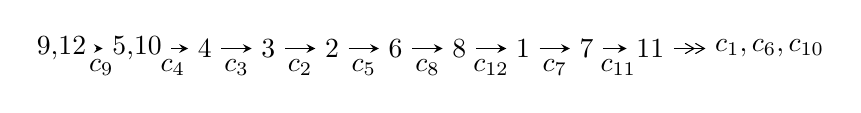
\begin{tikzpicture}[x=23pt, y=7pt]
	% node
	\node (A0) at (-1/8, 0) {9,12};
	\node (A1) at (17/16, 0) {5,10};
	\node (A2) at (17/8, 0) {4};
	\node (A3) at (25/8, 0) {3};
	\node (A4) at (33/8, 0) {2};
	\node (A5) at (41/8, 0) {6};
	\node (A6) at (49/8, 0) {8};
	\node (A7) at (57/8, 0) {1};
	\node (A8) at (65/8, 0) {7};
	\node (A9) at (73/8, 0) {11};
	\node (C1) at (1/2, -1) {$c_{9}$};
	\node (C2) at (13/8, -1) {$c_{4}$};
	\node (C3) at (21/8, -1) {$c_{3}$};
	\node (C4) at (29/8, -1) {$c_{2}$};
	\node (C5) at (37/8, -1) {$c_{5}$};
	\node (C6) at (45/8, -1) {$c_{8}$};
	\node (C7) at (53/8, -1) {$c_{12}$};
	\node (C8) at (61/8, -1) {$c_{7}$};
	\node (C9) at (69/8, -1) {$c_{11}$};
	\node (A10) at (11, 0) {$c_{1},c_{6},c_{10}$};

	% edge
	\draw[->,>=stealth]	
	(A0) edge (A1) (A1) edge (A2) (A2) edge (A3) (A3) edge (A4) (A4) edge (A5) (A5) edge (A6) (A6) edge (A7) (A7) edge (A8) (A8) edge (A9) ;
	\draw[->>,>={angle 60}]	
	(A9) edge (A10);
\end{tikzpicture} \\ 

\end{tabular} \\

\footnotetext{
The image of knot diagram is generated by the software ``\textbf{Draw programme}" developed by Andrew Bartholomew(\url{http://www.layer8.co.uk/maths/draw/index.htm\#Running-draw}), where we modified some parts for our purpose(\url{https://github.com/CATsTAILs/LinksPainter}).
}\phantom \\ \newline 
\centering \textbf{Ideals for irreducible components\footnotemark of $X_{\text{par}}$} 
 
\begin{align*}
I^u_{1}&=\langle 
5.47377\times10^{153} u^{62}-1.31028\times10^{154} u^{61}+\cdots+3.40987\times10^{153} b-1.11096\times10^{154},\\
\phantom{I^u_{1}}&\phantom{= \langle  }-1.23420\times10^{154} u^{62}+3.17083\times10^{154} u^{61}+\cdots+3.40987\times10^{153} a+7.52944\times10^{153},\\
\phantom{I^u_{1}}&\phantom{= \langle  }u^{63}-3 u^{62}+\cdots-2 u+1\rangle \\
I^u_{2}&=\langle 
1.49872\times10^{24} u^{27}+8.28499\times10^{24} u^{26}+\cdots+1.24369\times10^{24} b+2.46098\times10^{24},\\
\phantom{I^u_{2}}&\phantom{= \langle  }4.65953\times10^{23} u^{27}+2.34056\times10^{24} u^{26}+\cdots+1.24369\times10^{24} a-2.67968\times10^{24},\;u^{28}+6 u^{27}+\cdots+2 u+1\rangle \\
\\
\end{align*}
\raggedright * 2 irreducible components of $\dim_{\mathbb{C}}=0$, with total 91 representations.\\
\footnotetext{All coefficients of polynomials are rational numbers. But the coefficients are sometimes approximated in decimal forms when there is not enough margin.}
\newpage
\renewcommand{\arraystretch}{1}
\centering \section*{I. $I^u_{1}= \langle 5.47\times10^{153} u^{62}-1.31\times10^{154} u^{61}+\cdots+3.41\times10^{153} b-1.11\times10^{154},\;-1.23\times10^{154} u^{62}+3.17\times10^{154} u^{61}+\cdots+3.41\times10^{153} a+7.53\times10^{153},\;u^{63}-3 u^{62}+\cdots-2 u+1 \rangle$}
\flushleft \textbf{(i) Arc colorings}\\
\begin{tabular}{m{7pt} m{180pt} m{7pt} m{180pt} }
\flushright $a_{9}=$&$\begin{pmatrix}1\\0\end{pmatrix}$ \\
\flushright $a_{12}=$&$\begin{pmatrix}0\\u\end{pmatrix}$ \\
\flushright $a_{5}=$&$\begin{pmatrix}3.61950 u^{62}-9.29897 u^{61}+\cdots-13.6429 u-2.20813\\-1.60527 u^{62}+3.84260 u^{61}+\cdots+0.655818 u+3.25806\end{pmatrix}$ \\
\flushright $a_{10}=$&$\begin{pmatrix}1\\- u^2\end{pmatrix}$ \\
\flushright $a_{4}=$&$\begin{pmatrix}2.01423 u^{62}-5.45637 u^{61}+\cdots-12.9870 u+1.04993\\-1.60527 u^{62}+3.84260 u^{61}+\cdots+0.655818 u+3.25806\end{pmatrix}$ \\
\flushright $a_{3}=$&$\begin{pmatrix}3.54024 u^{62}-9.21354 u^{61}+\cdots-12.8013 u-1.62182\\-2.02759 u^{62}+4.91478 u^{61}+\cdots+0.540061 u+4.07895\end{pmatrix}$ \\
\flushright $a_{2}=$&$\begin{pmatrix}3.74628 u^{62}-11.2722 u^{61}+\cdots-3.10623 u+2.72252\\-1.51679 u^{62}+3.81152 u^{61}+\cdots+1.37033 u+1.85130\end{pmatrix}$ \\
\flushright $a_{6}=$&$\begin{pmatrix}2.19593 u^{62}-6.52686 u^{61}+\cdots+43.5636 u-10.7702\\-1.13065 u^{62}+2.95970 u^{61}+\cdots-2.68920 u+1.83845\end{pmatrix}$ \\
\flushright $a_{8}=$&$\begin{pmatrix}-2.38714 u^{62}+6.56354 u^{61}+\cdots+1.89950 u-0.514982\\1.03714 u^{62}-2.42670 u^{61}+\cdots-2.07634 u-1.29115\end{pmatrix}$ \\
\flushright $a_{1}=$&$\begin{pmatrix}1.65476 u^{62}-5.01519 u^{61}+\cdots+39.9437 u-9.20657\\-1.68517 u^{62}+4.43717 u^{61}+\cdots-3.41249 u+3.07668\end{pmatrix}$ \\
\flushright $a_{7}=$&$\begin{pmatrix}-1.57756 u^{62}+3.19097 u^{61}+\cdots+25.5743 u-0.805183\\0.777466 u^{62}-1.73082 u^{61}+\cdots-1.37482 u-1.84107\end{pmatrix}$ \\
\flushright $a_{11}=$&$\begin{pmatrix}-3.47962 u^{62}+11.2423 u^{61}+\cdots+14.4544 u-6.72853\\0.0868469 u^{62}-0.443124 u^{61}+\cdots-4.50613 u+1.35000\end{pmatrix}$\\&\end{tabular}
\flushleft \textbf{(ii) Obstruction class $= -1$}\\~\\
\flushleft \textbf{(iii) Cusp Shapes $= -4.27944 u^{62}+11.2388 u^{61}+\cdots+21.3904 u+3.08407$}\\~\\
\newpage\renewcommand{\arraystretch}{1}
\flushleft \textbf{(iv) u-Polynomials at the component}\newline \\
\begin{tabular}{m{50pt}|m{274pt}}
Crossings & \hspace{64pt}u-Polynomials at each crossing \\
\hline $$\begin{aligned}c_{1}\end{aligned}$$&$\begin{aligned}
&u^{63}+84 u^{62}+\cdots+6421262 u-290521
\end{aligned}$\\
\hline $$\begin{aligned}c_{2},c_{5}\end{aligned}$$&$\begin{aligned}
&u^{63}+42 u^{61}+\cdots+9624 u-539
\end{aligned}$\\
\hline $$\begin{aligned}c_{3}\end{aligned}$$&$\begin{aligned}
&u^{63}+u^{62}+\cdots+41175 u-7877
\end{aligned}$\\
\hline $$\begin{aligned}c_{4},c_{8}\end{aligned}$$&$\begin{aligned}
&u^{63}+3 u^{62}+\cdots-596 u-79
\end{aligned}$\\
\hline $$\begin{aligned}c_{6},c_{10}\end{aligned}$$&$\begin{aligned}
&u^{63}- u^{62}+\cdots-237 u-113
\end{aligned}$\\
\hline $$\begin{aligned}c_{7}\end{aligned}$$&$\begin{aligned}
&u^{63}+2 u^{62}+\cdots+3704 u-3077
\end{aligned}$\\
\hline $$\begin{aligned}c_{9}\end{aligned}$$&$\begin{aligned}
&u^{63}+3 u^{62}+\cdots-2 u-1
\end{aligned}$\\
\hline $$\begin{aligned}c_{11}\end{aligned}$$&$\begin{aligned}
&u^{63}-5 u^{62}+\cdots-6392 u-811
\end{aligned}$\\
\hline $$\begin{aligned}c_{12}\end{aligned}$$&$\begin{aligned}
&u^{63}- u^{62}+\cdots+39596508 u-17977599
\end{aligned}$\\
\hline
\end{tabular}\\~\\
\newpage\renewcommand{\arraystretch}{1}
\flushleft \textbf{(v) Riley Polynomials at the component}\newline \\
\begin{tabular}{m{50pt}|m{274pt}}
Crossings & \hspace{64pt}Riley Polynomials at each crossing \\
\hline $$\begin{aligned}c_{1}\end{aligned}$$&$\begin{aligned}
&y^{63}-188 y^{62}+\cdots+31966757369702 y-84402451441
\end{aligned}$\\
\hline $$\begin{aligned}c_{2},c_{5}\end{aligned}$$&$\begin{aligned}
&y^{63}+84 y^{62}+\cdots+6421262 y-290521
\end{aligned}$\\
\hline $$\begin{aligned}c_{3}\end{aligned}$$&$\begin{aligned}
&y^{63}+27 y^{62}+\cdots-719912377 y-62047129
\end{aligned}$\\
\hline $$\begin{aligned}c_{4},c_{8}\end{aligned}$$&$\begin{aligned}
&y^{63}+27 y^{62}+\cdots+125010 y-6241
\end{aligned}$\\
\hline $$\begin{aligned}c_{6},c_{10}\end{aligned}$$&$\begin{aligned}
&y^{63}+49 y^{62}+\cdots-228139 y-12769
\end{aligned}$\\
\hline $$\begin{aligned}c_{7}\end{aligned}$$&$\begin{aligned}
&y^{63}+94 y^{62}+\cdots-340978482 y-9467929
\end{aligned}$\\
\hline $$\begin{aligned}c_{9}\end{aligned}$$&$\begin{aligned}
&y^{63}-7 y^{62}+\cdots+2 y-1
\end{aligned}$\\
\hline $$\begin{aligned}c_{11}\end{aligned}$$&$\begin{aligned}
&y^{63}+3 y^{62}+\cdots+494194 y-657721
\end{aligned}$\\
\hline $$\begin{aligned}c_{12}\end{aligned}$$&$\begin{aligned}
&y^{63}+111 y^{62}+\cdots-5213792993463072 y-323194065804801
\end{aligned}$\\
\hline
\end{tabular}\\~\\
\newpage\flushleft \textbf{(vi) Complex Volumes and Cusp Shapes}
$$\begin{array}{c|c|c}  
\text{Solutions to }I^u_{1}& \I (\text{vol} + \sqrt{-1}CS) & \text{Cusp shape}\\
 \hline 
\begin{aligned}
u &= -0.854897 + 0.532929 I \\
a &= -0.100050 - 1.334720 I \\
b &= \phantom{-}1.29417 + 1.60493 I\end{aligned}
 & -10.02610 - 5.81545 I & \phantom{-}3.97856 + 5.33947 I \\ \hline\begin{aligned}
u &= -0.854897 - 0.532929 I \\
a &= -0.100050 + 1.334720 I \\
b &= \phantom{-}1.29417 - 1.60493 I\end{aligned}
 & -10.02610 + 5.81545 I & \phantom{-}3.97856 - 5.33947 I \\ \hline\begin{aligned}
u &= \phantom{-}0.718348 + 0.648111 I \\
a &= \phantom{-}0.449487 + 1.049550 I \\
b &= -0.87436 - 1.40145 I\end{aligned}
 & -3.35191 + 2.65403 I & \phantom{-}2.16615 - 3.99621 I \\ \hline\begin{aligned}
u &= \phantom{-}0.718348 - 0.648111 I \\
a &= \phantom{-}0.449487 - 1.049550 I \\
b &= -0.87436 + 1.40145 I\end{aligned}
 & -3.35191 - 2.65403 I & \phantom{-}2.16615 + 3.99621 I \\ \hline\begin{aligned}
u &= -0.577833 + 0.736890 I \\
a &= \phantom{-}0.459738 + 0.125771 I \\
b &= \phantom{-}0.646165 + 0.254111 I\end{aligned}
 & -1.42068 - 2.29477 I & \phantom{-}3.60284 + 3.89630 I \\ \hline\begin{aligned}
u &= -0.577833 - 0.736890 I \\
a &= \phantom{-}0.459738 - 0.125771 I \\
b &= \phantom{-}0.646165 - 0.254111 I\end{aligned}
 & -1.42068 + 2.29477 I & \phantom{-}3.60284 - 3.89630 I \\ \hline\begin{aligned}
u &= -0.384316 + 1.017510 I \\
a &= -0.775849 - 0.891790 I \\
b &= \phantom{-}0.619662 - 1.136280 I\end{aligned}
 & -11.98870 + 1.15184 I & \phantom{-0.000000 } 0 \\ \hline\begin{aligned}
u &= -0.384316 - 1.017510 I \\
a &= -0.775849 + 0.891790 I \\
b &= \phantom{-}0.619662 + 1.136280 I\end{aligned}
 & -11.98870 - 1.15184 I & \phantom{-0.000000 } 0 \\ \hline\begin{aligned}
u &= \phantom{-}0.012682 + 1.109030 I \\
a &= -0.273611 + 0.515935 I \\
b &= -0.344619 + 0.593299 I\end{aligned}
 & -4.43543 - 0.90885 I & \phantom{-0.000000 } 0 \\ \hline\begin{aligned}
u &= \phantom{-}0.012682 - 1.109030 I \\
a &= -0.273611 - 0.515935 I \\
b &= -0.344619 - 0.593299 I\end{aligned}
 & -4.43543 + 0.90885 I & \phantom{-0.000000 } 0\\
 \hline 
 \end{array}$$\newpage$$\begin{array}{c|c|c}  
\text{Solutions to }I^u_{1}& \I (\text{vol} + \sqrt{-1}CS) & \text{Cusp shape}\\
 \hline 
\begin{aligned}
u &= \phantom{-}0.695265 + 0.873390 I \\
a &= -0.668200 - 0.224791 I \\
b &= \phantom{-}1.78864 + 0.50256 I\end{aligned}
 & -16.4493 + 6.5283 I & \phantom{-0.000000 } 0 \\ \hline\begin{aligned}
u &= \phantom{-}0.695265 - 0.873390 I \\
a &= -0.668200 + 0.224791 I \\
b &= \phantom{-}1.78864 - 0.50256 I\end{aligned}
 & -16.4493 - 6.5283 I & \phantom{-0.000000 } 0 \\ \hline\begin{aligned}
u &= \phantom{-}0.711162 + 0.860779 I \\
a &= -0.608050 - 0.358721 I \\
b &= -0.773545 + 0.642592 I\end{aligned}
 & -3.49757 + 7.28817 I & \phantom{-0.000000 } 0 \\ \hline\begin{aligned}
u &= \phantom{-}0.711162 - 0.860779 I \\
a &= -0.608050 + 0.358721 I \\
b &= -0.773545 - 0.642592 I\end{aligned}
 & -3.49757 - 7.28817 I & \phantom{-0.000000 } 0 \\ \hline\begin{aligned}
u &= \phantom{-}0.152045 + 1.129920 I \\
a &= \phantom{-}0.543142 - 0.504864 I \\
b &= -0.517588 - 0.574682 I\end{aligned}
 & -8.52986 - 1.24389 I & \phantom{-0.000000 } 0 \\ \hline\begin{aligned}
u &= \phantom{-}0.152045 - 1.129920 I \\
a &= \phantom{-}0.543142 + 0.504864 I \\
b &= -0.517588 + 0.574682 I\end{aligned}
 & -8.52986 + 1.24389 I & \phantom{-0.000000 } 0 \\ \hline\begin{aligned}
u &= \phantom{-}0.927854 + 0.686316 I \\
a &= \phantom{-}0.129275 + 0.765769 I \\
b &= \phantom{-}0.790898 - 0.247331 I\end{aligned}
 & -2.96009 + 2.72627 I & \phantom{-0.000000 } 0 \\ \hline\begin{aligned}
u &= \phantom{-}0.927854 - 0.686316 I \\
a &= \phantom{-}0.129275 - 0.765769 I \\
b &= \phantom{-}0.790898 + 0.247331 I\end{aligned}
 & -2.96009 - 2.72627 I & \phantom{-0.000000 } 0 \\ \hline\begin{aligned}
u &= \phantom{-}0.811068 + 0.821995 I \\
a &= \phantom{-}1.20206 + 1.10469 I \\
b &= \phantom{-}0.385751 - 1.186730 I\end{aligned}
 & \phantom{-}0.74682 + 6.31225 I & \phantom{-0.000000 } 0 \\ \hline\begin{aligned}
u &= \phantom{-}0.811068 - 0.821995 I \\
a &= \phantom{-}1.20206 - 1.10469 I \\
b &= \phantom{-}0.385751 + 1.186730 I\end{aligned}
 & \phantom{-}0.74682 - 6.31225 I & \phantom{-0.000000 } 0\\
 \hline 
 \end{array}$$\newpage$$\begin{array}{c|c|c}  
\text{Solutions to }I^u_{1}& \I (\text{vol} + \sqrt{-1}CS) & \text{Cusp shape}\\
 \hline 
\begin{aligned}
u &= -0.614787 + 0.470038 I \\
a &= \phantom{-}1.118150 + 0.859293 I \\
b &= \phantom{-}0.237265 - 0.057936 I\end{aligned}
 & -1.33985 - 2.52478 I & \phantom{-}5.87677 + 6.20065 I \\ \hline\begin{aligned}
u &= -0.614787 - 0.470038 I \\
a &= \phantom{-}1.118150 - 0.859293 I \\
b &= \phantom{-}0.237265 + 0.057936 I\end{aligned}
 & -1.33985 + 2.52478 I & \phantom{-}5.87677 - 6.20065 I \\ \hline\begin{aligned}
u &= \phantom{-}0.606281 + 0.460474 I \\
a &= -0.11967 - 1.89327 I \\
b &= -0.80135 + 1.17152 I\end{aligned}
 & -6.06901 + 4.19971 I & \phantom{-}0.46981 + 4.89096 I \\ \hline\begin{aligned}
u &= \phantom{-}0.606281 - 0.460474 I \\
a &= -0.11967 + 1.89327 I \\
b &= -0.80135 - 1.17152 I\end{aligned}
 & -6.06901 - 4.19971 I & \phantom{-}0.46981 - 4.89096 I \\ \hline\begin{aligned}
u &= \phantom{-}0.742696 + 0.018030 I \\
a &= \phantom{-}0.802844 - 0.672931 I \\
b &= \phantom{-}0.123330 - 0.408590 I\end{aligned}
 & -2.29683 - 3.13725 I & \phantom{-}3.03113 + 2.28651 I \\ \hline\begin{aligned}
u &= \phantom{-}0.742696 - 0.018030 I \\
a &= \phantom{-}0.802844 + 0.672931 I \\
b &= \phantom{-}0.123330 + 0.408590 I\end{aligned}
 & -2.29683 + 3.13725 I & \phantom{-}3.03113 - 2.28651 I \\ \hline\begin{aligned}
u &= \phantom{-}1.157620 + 0.544016 I \\
a &= -0.53473 + 2.17350 I \\
b &= \phantom{-}0.888311 - 0.750993 I\end{aligned}
 & -14.8647 - 0.9237 I & \phantom{-0.000000 } 0 \\ \hline\begin{aligned}
u &= \phantom{-}1.157620 - 0.544016 I \\
a &= -0.53473 - 2.17350 I \\
b &= \phantom{-}0.888311 + 0.750993 I\end{aligned}
 & -14.8647 + 0.9237 I & \phantom{-0.000000 } 0 \\ \hline\begin{aligned}
u &= -0.679644 + 0.115394 I \\
a &= -0.016821 + 0.810279 I \\
b &= -1.298680 - 0.546785 I\end{aligned}
 & -0.552090 - 1.157580 I & \phantom{-}8.72526 + 2.52584 I \\ \hline\begin{aligned}
u &= -0.679644 - 0.115394 I \\
a &= -0.016821 - 0.810279 I \\
b &= -1.298680 + 0.546785 I\end{aligned}
 & -0.552090 + 1.157580 I & \phantom{-}8.72526 - 2.52584 I\\
 \hline 
 \end{array}$$\newpage$$\begin{array}{c|c|c}  
\text{Solutions to }I^u_{1}& \I (\text{vol} + \sqrt{-1}CS) & \text{Cusp shape}\\
 \hline 
\begin{aligned}
u &= \phantom{-}1.044930 + 0.812912 I \\
a &= -0.75989 - 1.82673 I \\
b &= -0.442668 + 1.276840 I\end{aligned}
 & -2.69001 + 2.91714 I & \phantom{-0.000000 } 0 \\ \hline\begin{aligned}
u &= \phantom{-}1.044930 - 0.812912 I \\
a &= -0.75989 + 1.82673 I \\
b &= -0.442668 - 1.276840 I\end{aligned}
 & -2.69001 - 2.91714 I & \phantom{-0.000000 } 0 \\ \hline\begin{aligned}
u &= -1.11456 + 0.87594 I \\
a &= -0.584881 + 1.062470 I \\
b &= -0.301834 - 1.243090 I\end{aligned}
 & \phantom{-}4.07431 - 2.64903 I & \phantom{-0.000000 } 0 \\ \hline\begin{aligned}
u &= -1.11456 - 0.87594 I \\
a &= -0.584881 - 1.062470 I \\
b &= -0.301834 + 1.243090 I\end{aligned}
 & \phantom{-}4.07431 + 2.64903 I & \phantom{-0.000000 } 0 \\ \hline\begin{aligned}
u &= \phantom{-}0.73967 + 1.23237 I \\
a &= \phantom{-}0.234778 + 0.158687 I \\
b &= -0.732813 - 0.431119 I\end{aligned}
 & -5.61316 - 1.82436 I & \phantom{-0.000000 } 0 \\ \hline\begin{aligned}
u &= \phantom{-}0.73967 - 1.23237 I \\
a &= \phantom{-}0.234778 - 0.158687 I \\
b &= -0.732813 + 0.431119 I\end{aligned}
 & -5.61316 + 1.82436 I & \phantom{-0.000000 } 0 \\ \hline\begin{aligned}
u &= \phantom{-}0.489917 + 0.265929 I \\
a &= -0.631980 - 1.069290 I \\
b &= \phantom{-}0.17708 + 1.44057 I\end{aligned}
 & \phantom{-}0.77156 - 1.96953 I & \phantom{-}11.39719 + 1.23723 I \\ \hline\begin{aligned}
u &= \phantom{-}0.489917 - 0.265929 I \\
a &= -0.631980 + 1.069290 I \\
b &= \phantom{-}0.17708 - 1.44057 I\end{aligned}
 & \phantom{-}0.77156 + 1.96953 I & \phantom{-}11.39719 - 1.23723 I \\ \hline\begin{aligned}
u &= -0.69545 + 1.27793 I \\
a &= \phantom{-}0.589761 - 0.467742 I \\
b &= -1.013060 + 0.642851 I\end{aligned}
 & -10.25240 - 0.58456 I & \phantom{-0.000000 } 0 \\ \hline\begin{aligned}
u &= -0.69545 - 1.27793 I \\
a &= \phantom{-}0.589761 + 0.467742 I \\
b &= -1.013060 - 0.642851 I\end{aligned}
 & -10.25240 + 0.58456 I & \phantom{-0.000000 } 0\\
 \hline 
 \end{array}$$\newpage$$\begin{array}{c|c|c}  
\text{Solutions to }I^u_{1}& \I (\text{vol} + \sqrt{-1}CS) & \text{Cusp shape}\\
 \hline 
\begin{aligned}
u &= -0.528848\phantom{ +0.000000I} \\
a &= -0.754706\phantom{ +0.000000I} \\
b &= -0.350552\phantom{ +0.000000I}\end{aligned}
 & \phantom{-}0.833691\phantom{ +0.000000I} & \phantom{-}12.5370\phantom{ +0.000000I} \\ \hline\begin{aligned}
u &= \phantom{-}1.17530 + 0.94653 I \\
a &= -0.099026 - 1.222920 I \\
b &= -0.902120 + 0.943721 I\end{aligned}
 & -4.22732 + 9.52870 I & \phantom{-0.000000 } 0 \\ \hline\begin{aligned}
u &= \phantom{-}1.17530 - 0.94653 I \\
a &= -0.099026 + 1.222920 I \\
b &= -0.902120 - 0.943721 I\end{aligned}
 & -4.22732 - 9.52870 I & \phantom{-0.000000 } 0 \\ \hline\begin{aligned}
u &= \phantom{-}0.469414 + 0.086831 I \\
a &= -0.24275 + 2.14834 I \\
b &= \phantom{-}0.304078 - 1.019980 I\end{aligned}
 & \phantom{-}0.75672 + 1.60252 I & \phantom{-}5.44397 - 2.96352 I \\ \hline\begin{aligned}
u &= \phantom{-}0.469414 - 0.086831 I \\
a &= -0.24275 - 2.14834 I \\
b &= \phantom{-}0.304078 + 1.019980 I\end{aligned}
 & \phantom{-}0.75672 - 1.60252 I & \phantom{-}5.44397 + 2.96352 I \\ \hline\begin{aligned}
u &= \phantom{-}1.11667 + 1.07117 I \\
a &= \phantom{-}0.32680 + 1.51043 I \\
b &= \phantom{-}0.91203 - 1.47375 I\end{aligned}
 & -13.1892 + 15.5433 I & \phantom{-0.000000 } 0 \\ \hline\begin{aligned}
u &= \phantom{-}1.11667 - 1.07117 I \\
a &= \phantom{-}0.32680 - 1.51043 I \\
b &= \phantom{-}0.91203 + 1.47375 I\end{aligned}
 & -13.1892 - 15.5433 I & \phantom{-0.000000 } 0 \\ \hline\begin{aligned}
u &= -0.040555 + 0.445575 I \\
a &= -2.19312 + 1.06421 I \\
b &= -0.162171 - 1.085770 I\end{aligned}
 & -2.67022 - 3.59787 I & \phantom{-}1.26601 + 4.62354 I \\ \hline\begin{aligned}
u &= -0.040555 - 0.445575 I \\
a &= -2.19312 - 1.06421 I \\
b &= -0.162171 + 1.085770 I\end{aligned}
 & -2.67022 + 3.59787 I & \phantom{-}1.26601 - 4.62354 I \\ \hline\begin{aligned}
u &= -1.06557 + 1.17893 I \\
a &= \phantom{-}0.465568 - 0.962520 I \\
b &= \phantom{-}0.214621 + 1.324260 I\end{aligned}
 & \phantom{-}3.14454 - 5.28865 I & \phantom{-0.000000 } 0\\
 \hline 
 \end{array}$$\newpage$$\begin{array}{c|c|c}  
\text{Solutions to }I^u_{1}& \I (\text{vol} + \sqrt{-1}CS) & \text{Cusp shape}\\
 \hline 
\begin{aligned}
u &= -1.06557 - 1.17893 I \\
a &= \phantom{-}0.465568 + 0.962520 I \\
b &= \phantom{-}0.214621 - 1.324260 I\end{aligned}
 & \phantom{-}3.14454 + 5.28865 I & \phantom{-0.000000 } 0 \\ \hline\begin{aligned}
u &= -1.54201 + 0.46506 I \\
a &= -0.40850 + 1.52127 I \\
b &= -0.000517 - 1.179550 I\end{aligned}
 & \phantom{-}4.85414 - 2.03164 I & \phantom{-0.000000 } 0 \\ \hline\begin{aligned}
u &= -1.54201 - 0.46506 I \\
a &= -0.40850 - 1.52127 I \\
b &= -0.000517 + 1.179550 I\end{aligned}
 & \phantom{-}4.85414 + 2.03164 I & \phantom{-0.000000 } 0 \\ \hline\begin{aligned}
u &= -1.27163 + 0.99225 I \\
a &= -0.00808 + 1.62331 I \\
b &= -0.84144 - 1.21606 I\end{aligned}
 & -8.48368 - 7.48858 I & \phantom{-0.000000 } 0 \\ \hline\begin{aligned}
u &= -1.27163 - 0.99225 I \\
a &= -0.00808 - 1.62331 I \\
b &= -0.84144 + 1.21606 I\end{aligned}
 & -8.48368 + 7.48858 I & \phantom{-0.000000 } 0 \\ \hline\begin{aligned}
u &= -0.160337 + 0.343315 I \\
a &= \phantom{-}0.339442 + 0.084802 I \\
b &= \phantom{-}0.614423 + 1.266600 I\end{aligned}
 & \phantom{-}0.79379 - 2.25708 I & \phantom{-}2.28794 - 4.37801 I \\ \hline\begin{aligned}
u &= -0.160337 - 0.343315 I \\
a &= \phantom{-}0.339442 - 0.084802 I \\
b &= \phantom{-}0.614423 - 1.266600 I\end{aligned}
 & \phantom{-}0.79379 + 2.25708 I & \phantom{-}2.28794 + 4.37801 I \\ \hline\begin{aligned}
u &= \phantom{-}1.09583 + 1.21738 I \\
a &= -0.710263 - 0.627589 I \\
b &= \phantom{-}0.779094 + 1.174620 I\end{aligned}
 & -13.4744 - 7.2599 I & \phantom{-0.000000 } 0 \\ \hline\begin{aligned}
u &= \phantom{-}1.09583 - 1.21738 I \\
a &= -0.710263 + 0.627589 I \\
b &= \phantom{-}0.779094 - 1.174620 I\end{aligned}
 & -13.4744 + 7.2599 I & \phantom{-0.000000 } 0 \\ \hline\begin{aligned}
u &= -0.234232 + 0.257654 I \\
a &= \phantom{-}0.62787 - 9.86711 I \\
b &= \phantom{-}0.571174 + 0.777335 I\end{aligned}
 & -13.25520 - 3.60698 I & \phantom{-}0.0981 + 14.8573 I\\
 \hline 
 \end{array}$$\newpage$$\begin{array}{c|c|c}  
\text{Solutions to }I^u_{1}& \I (\text{vol} + \sqrt{-1}CS) & \text{Cusp shape}\\
 \hline 
\begin{aligned}
u &= -0.234232 - 0.257654 I \\
a &= \phantom{-}0.62787 + 9.86711 I \\
b &= \phantom{-}0.571174 - 0.777335 I\end{aligned}
 & -13.25520 + 3.60698 I & \phantom{-}0.0981 - 14.8573 I \\ \hline\begin{aligned}
u &= -1.66651 + 0.55104 I \\
a &= -0.176083 - 0.957519 I \\
b &= \phantom{-}0.335346 + 0.557889 I\end{aligned}
 & \phantom{-}2.14723 - 3.04462 I & \phantom{-0.000000 } 0 \\ \hline\begin{aligned}
u &= -1.66651 - 0.55104 I \\
a &= -0.176083 + 0.957519 I \\
b &= \phantom{-}0.335346 - 0.557889 I\end{aligned}
 & \phantom{-}2.14723 + 3.04462 I & \phantom{-0.000000 } 0\\
 \hline 
 \end{array}$$\newpage\newpage\renewcommand{\arraystretch}{1}
\centering \section*{II. $I^u_{2}= \langle 1.50\times10^{24} u^{27}+8.28\times10^{24} u^{26}+\cdots+1.24\times10^{24} b+2.46\times10^{24},\;4.66\times10^{23} u^{27}+2.34\times10^{24} u^{26}+\cdots+1.24\times10^{24} a-2.68\times10^{24},\;u^{28}+6 u^{27}+\cdots+2 u+1 \rangle$}
\flushleft \textbf{(i) Arc colorings}\\
\begin{tabular}{m{7pt} m{180pt} m{7pt} m{180pt} }
\flushright $a_{9}=$&$\begin{pmatrix}1\\0\end{pmatrix}$ \\
\flushright $a_{12}=$&$\begin{pmatrix}0\\u\end{pmatrix}$ \\
\flushright $a_{5}=$&$\begin{pmatrix}-0.374654 u^{27}-1.88195 u^{26}+\cdots+6.62313 u+2.15462\\-1.20506 u^{27}-6.66162 u^{26}+\cdots-3.47743 u-1.97877\end{pmatrix}$ \\
\flushright $a_{10}=$&$\begin{pmatrix}1\\- u^2\end{pmatrix}$ \\
\flushright $a_{4}=$&$\begin{pmatrix}-1.57971 u^{27}-8.54357 u^{26}+\cdots+3.14570 u+0.175849\\-1.20506 u^{27}-6.66162 u^{26}+\cdots-3.47743 u-1.97877\end{pmatrix}$ \\
\flushright $a_{3}=$&$\begin{pmatrix}-0.347434 u^{27}-1.83630 u^{26}+\cdots+6.91281 u+3.08931\\-1.28412 u^{27}-7.15895 u^{26}+\cdots-3.61794 u-2.66516\end{pmatrix}$ \\
\flushright $a_{2}=$&$\begin{pmatrix}1.99908 u^{27}+12.7360 u^{26}+\cdots+6.48433 u+2.16177\\-0.842153 u^{27}-4.69396 u^{26}+\cdots-1.32507 u-0.0688727\end{pmatrix}$ \\
\flushright $a_{6}=$&$\begin{pmatrix}2.23949 u^{27}+13.0407 u^{26}+\cdots-12.3400 u-5.56425\\-0.585524 u^{27}-3.13244 u^{26}+\cdots+2.42745 u+0.356599\end{pmatrix}$ \\
\flushright $a_{8}=$&$\begin{pmatrix}0.260068 u^{27}+1.72336 u^{26}+\cdots+5.30274 u-0.950249\\0.0297660 u^{27}+0.579857 u^{26}+\cdots-1.78144 u+1.63844\end{pmatrix}$ \\
\flushright $a_{1}=$&$\begin{pmatrix}2.39626 u^{27}+14.6108 u^{26}+\cdots-17.2118 u-6.13078\\-0.395076 u^{27}-2.09431 u^{26}+\cdots+3.82248 u+0.336223\end{pmatrix}$ \\
\flushright $a_{7}=$&$\begin{pmatrix}-0.463227 u^{27}-3.40262 u^{26}+\cdots+8.77999 u+3.35500\\-0.00664464 u^{27}+0.175348 u^{26}+\cdots-2.87462 u+0.243559\end{pmatrix}$ \\
\flushright $a_{11}=$&$\begin{pmatrix}-1.26164 u^{27}-8.15989 u^{26}+\cdots-12.1726 u-0.310184\\0.564215 u^{27}+3.40566 u^{26}+\cdots+0.108528 u-0.289834\end{pmatrix}$\\&\end{tabular}
\flushleft \textbf{(ii) Obstruction class $= 1$}\\~\\
\flushleft \textbf{(iii) Cusp Shapes $= \frac{14196894526534098056419915}{1243689822254210224198313} u^{27}+\frac{77156772533747101068768450}{1243689822254210224198313} u^{26}+\cdots+\frac{18009890446390071079402793}{1243689822254210224198313} u+\frac{24155927693538196022412912}{1243689822254210224198313}$}\\~\\
\newpage\renewcommand{\arraystretch}{1}
\flushleft \textbf{(iv) u-Polynomials at the component}\newline \\
\begin{tabular}{m{50pt}|m{274pt}}
Crossings & \hspace{64pt}u-Polynomials at each crossing \\
\hline $$\begin{aligned}c_{1}\end{aligned}$$&$\begin{aligned}
&u^{28}-29 u^{27}+\cdots-336 u+25
\end{aligned}$\\
\hline $$\begin{aligned}c_{2}\end{aligned}$$&$\begin{aligned}
&u^{28}+3 u^{27}+\cdots+28 u+5
\end{aligned}$\\
\hline $$\begin{aligned}c_{3}\end{aligned}$$&$\begin{aligned}
&u^{28}+2 u^{26}+\cdots+u+1
\end{aligned}$\\
\hline $$\begin{aligned}c_{4}\end{aligned}$$&$\begin{aligned}
&u^{28}+12 u^{26}+\cdots+126 u^2+13
\end{aligned}$\\
\hline $$\begin{aligned}c_{5}\end{aligned}$$&$\begin{aligned}
&u^{28}-3 u^{27}+\cdots-28 u+5
\end{aligned}$\\
\hline $$\begin{aligned}c_{6}\end{aligned}$$&$\begin{aligned}
&u^{28}+7 u^{26}+\cdots+3 u+1
\end{aligned}$\\
\hline $$\begin{aligned}c_{7}\end{aligned}$$&$\begin{aligned}
&u^{28}+u^{27}+\cdots-238 u+79
\end{aligned}$\\
\hline $$\begin{aligned}c_{8}\end{aligned}$$&$\begin{aligned}
&u^{28}+12 u^{26}+\cdots+126 u^2+13
\end{aligned}$\\
\hline $$\begin{aligned}c_{9}\end{aligned}$$&$\begin{aligned}
&u^{28}+6 u^{27}+\cdots+2 u+1
\end{aligned}$\\
\hline $$\begin{aligned}c_{10}\end{aligned}$$&$\begin{aligned}
&u^{28}+7 u^{26}+\cdots-3 u+1
\end{aligned}$\\
\hline $$\begin{aligned}c_{11}\end{aligned}$$&$\begin{aligned}
&u^{28}-4 u^{26}+\cdots+2 u+1
\end{aligned}$\\
\hline $$\begin{aligned}c_{12}\end{aligned}$$&$\begin{aligned}
&u^{28}+6 u^{26}+\cdots-6 u+1
\end{aligned}$\\
\hline
\end{tabular}\\~\\
\newpage\renewcommand{\arraystretch}{1}
\flushleft \textbf{(v) Riley Polynomials at the component}\newline \\
\begin{tabular}{m{50pt}|m{274pt}}
Crossings & \hspace{64pt}Riley Polynomials at each crossing \\
\hline $$\begin{aligned}c_{1}\end{aligned}$$&$\begin{aligned}
&y^{28}-39 y^{27}+\cdots+18404 y+625
\end{aligned}$\\
\hline $$\begin{aligned}c_{2},c_{5}\end{aligned}$$&$\begin{aligned}
&y^{28}+29 y^{27}+\cdots+336 y+25
\end{aligned}$\\
\hline $$\begin{aligned}c_{3}\end{aligned}$$&$\begin{aligned}
&y^{28}+4 y^{27}+\cdots+23 y+1
\end{aligned}$\\
\hline $$\begin{aligned}c_{4},c_{8}\end{aligned}$$&$\begin{aligned}
&y^{28}+24 y^{27}+\cdots+3276 y+169
\end{aligned}$\\
\hline $$\begin{aligned}c_{6},c_{10}\end{aligned}$$&$\begin{aligned}
&y^{28}+14 y^{27}+\cdots+17 y+1
\end{aligned}$\\
\hline $$\begin{aligned}c_{7}\end{aligned}$$&$\begin{aligned}
&y^{28}+31 y^{27}+\cdots+69440 y+6241
\end{aligned}$\\
\hline $$\begin{aligned}c_{9}\end{aligned}$$&$\begin{aligned}
&y^{28}-6 y^{27}+\cdots-8 y+1
\end{aligned}$\\
\hline $$\begin{aligned}c_{11}\end{aligned}$$&$\begin{aligned}
&y^{28}-8 y^{27}+\cdots+16 y+1
\end{aligned}$\\
\hline $$\begin{aligned}c_{12}\end{aligned}$$&$\begin{aligned}
&y^{28}+12 y^{27}+\cdots-14 y+1
\end{aligned}$\\
\hline
\end{tabular}\\~\\
\newpage\flushleft \textbf{(vi) Complex Volumes and Cusp Shapes}
$$\begin{array}{c|c|c}  
\text{Solutions to }I^u_{2}& \I (\text{vol} + \sqrt{-1}CS) & \text{Cusp shape}\\
 \hline 
\begin{aligned}
u &= \phantom{-}0.940292 + 0.413387 I \\
a &= \phantom{-}1.23072 + 2.12971 I \\
b &= \phantom{-}0.300613 - 1.070080 I\end{aligned}
 & -1.05959 + 4.61100 I & \phantom{-}6.51158 - 5.52677 I \\ \hline\begin{aligned}
u &= \phantom{-}0.940292 - 0.413387 I \\
a &= \phantom{-}1.23072 - 2.12971 I \\
b &= \phantom{-}0.300613 + 1.070080 I\end{aligned}
 & -1.05959 - 4.61100 I & \phantom{-}6.51158 + 5.52677 I \\ \hline\begin{aligned}
u &= \phantom{-}0.806078 + 0.496313 I \\
a &= \phantom{-}0.083024 + 0.969496 I \\
b &= \phantom{-}0.175391 - 1.342910 I\end{aligned}
 & -0.16211 - 1.47199 I & \phantom{-}4.14534 - 0.40207 I \\ \hline\begin{aligned}
u &= \phantom{-}0.806078 - 0.496313 I \\
a &= \phantom{-}0.083024 - 0.969496 I \\
b &= \phantom{-}0.175391 + 1.342910 I\end{aligned}
 & -0.16211 + 1.47199 I & \phantom{-}4.14534 + 0.40207 I \\ \hline\begin{aligned}
u &= -0.653575 + 0.631653 I \\
a &= \phantom{-}0.16569 - 1.53605 I \\
b &= \phantom{-}0.85490 + 1.21262 I\end{aligned}
 & -5.97610 - 4.67435 I & \phantom{-}3.55527 + 10.86527 I \\ \hline\begin{aligned}
u &= -0.653575 - 0.631653 I \\
a &= \phantom{-}0.16569 + 1.53605 I \\
b &= \phantom{-}0.85490 - 1.21262 I\end{aligned}
 & -5.97610 + 4.67435 I & \phantom{-}3.55527 - 10.86527 I \\ \hline\begin{aligned}
u &= \phantom{-}0.217968 + 1.154320 I \\
a &= -0.564796 + 0.248293 I \\
b &= -0.066810 + 0.479178 I\end{aligned}
 & -4.21962 - 1.45210 I & \phantom{-}5.81625 + 6.66607 I \\ \hline\begin{aligned}
u &= \phantom{-}0.217968 - 1.154320 I \\
a &= -0.564796 - 0.248293 I \\
b &= -0.066810 - 0.479178 I\end{aligned}
 & -4.21962 + 1.45210 I & \phantom{-}5.81625 - 6.66607 I \\ \hline\begin{aligned}
u &= -0.216540 + 1.244680 I \\
a &= -0.414021 - 0.246811 I \\
b &= \phantom{-}0.522371 - 0.713383 I\end{aligned}
 & -8.29018 + 0.47114 I & \phantom{-}3.38775 + 2.13311 I \\ \hline\begin{aligned}
u &= -0.216540 - 1.244680 I \\
a &= -0.414021 + 0.246811 I \\
b &= \phantom{-}0.522371 + 0.713383 I\end{aligned}
 & -8.29018 - 0.47114 I & \phantom{-}3.38775 - 2.13311 I\\
 \hline 
 \end{array}$$\newpage$$\begin{array}{c|c|c}  
\text{Solutions to }I^u_{2}& \I (\text{vol} + \sqrt{-1}CS) & \text{Cusp shape}\\
 \hline 
\begin{aligned}
u &= \phantom{-}0.622908 + 0.349779 I \\
a &= -0.216133 + 1.033420 I \\
b &= -0.632440 - 1.103600 I\end{aligned}
 & -1.58788 + 4.47956 I & \phantom{-}8.31123 - 10.39210 I \\ \hline\begin{aligned}
u &= \phantom{-}0.622908 - 0.349779 I \\
a &= -0.216133 - 1.033420 I \\
b &= -0.632440 + 1.103600 I\end{aligned}
 & -1.58788 - 4.47956 I & \phantom{-}8.31123 + 10.39210 I \\ \hline\begin{aligned}
u &= \phantom{-}0.926454 + 0.990307 I \\
a &= -1.014490 - 0.881408 I \\
b &= -0.219668 + 1.137670 I\end{aligned}
 & -0.67708 + 7.39786 I & \phantom{-}3.61944 - 6.76047 I \\ \hline\begin{aligned}
u &= \phantom{-}0.926454 - 0.990307 I \\
a &= -1.014490 + 0.881408 I \\
b &= -0.219668 - 1.137670 I\end{aligned}
 & -0.67708 - 7.39786 I & \phantom{-}3.61944 + 6.76047 I \\ \hline\begin{aligned}
u &= -1.104760 + 0.873270 I \\
a &= -0.517047 + 1.068910 I \\
b &= -0.355700 - 1.347290 I\end{aligned}
 & \phantom{-}3.39497 - 2.92110 I & \phantom{-}2.45276 + 2.72271 I \\ \hline\begin{aligned}
u &= -1.104760 - 0.873270 I \\
a &= -0.517047 - 1.068910 I \\
b &= -0.355700 + 1.347290 I\end{aligned}
 & \phantom{-}3.39497 + 2.92110 I & \phantom{-}2.45276 - 2.72271 I \\ \hline\begin{aligned}
u &= -0.354078 + 0.377348 I \\
a &= \phantom{-}0.67911 + 1.78144 I \\
b &= \phantom{-}0.908649 - 0.411620 I\end{aligned}
 & -1.76047 - 1.65206 I & \phantom{-}2.39742 + 0.15868 I \\ \hline\begin{aligned}
u &= -0.354078 - 0.377348 I \\
a &= \phantom{-}0.67911 - 1.78144 I \\
b &= \phantom{-}0.908649 + 0.411620 I\end{aligned}
 & -1.76047 + 1.65206 I & \phantom{-}2.39742 - 0.15868 I \\ \hline\begin{aligned}
u &= -0.462042 + 0.226447 I \\
a &= -0.364429 + 1.069470 I \\
b &= -0.86212 - 1.27313 I\end{aligned}
 & \phantom{-}0.99320 - 2.56181 I & \phantom{-}15.9971 + 14.1165 I \\ \hline\begin{aligned}
u &= -0.462042 - 0.226447 I \\
a &= -0.364429 - 1.069470 I \\
b &= -0.86212 + 1.27313 I\end{aligned}
 & \phantom{-}0.99320 + 2.56181 I & \phantom{-}15.9971 - 14.1165 I\\
 \hline 
 \end{array}$$\newpage$$\begin{array}{c|c|c}  
\text{Solutions to }I^u_{2}& \I (\text{vol} + \sqrt{-1}CS) & \text{Cusp shape}\\
 \hline 
\begin{aligned}
u &= \phantom{-}0.377108 + 0.341592 I \\
a &= \phantom{-}5.78433 + 1.20797 I \\
b &= -0.590667 - 0.703657 I\end{aligned}
 & -13.21040 - 3.22197 I & \phantom{-}2.66915 - 5.24743 I \\ \hline\begin{aligned}
u &= \phantom{-}0.377108 - 0.341592 I \\
a &= \phantom{-}5.78433 - 1.20797 I \\
b &= -0.590667 + 0.703657 I\end{aligned}
 & -13.21040 + 3.22197 I & \phantom{-}2.66915 + 5.24743 I \\ \hline\begin{aligned}
u &= -1.00439 + 1.16349 I \\
a &= \phantom{-}0.580992 - 0.879373 I \\
b &= \phantom{-}0.199655 + 1.398360 I\end{aligned}
 & \phantom{-}2.49042 - 4.78963 I & \phantom{-}2.06444 + 2.28263 I \\ \hline\begin{aligned}
u &= -1.00439 - 1.16349 I \\
a &= \phantom{-}0.580992 + 0.879373 I \\
b &= \phantom{-}0.199655 - 1.398360 I\end{aligned}
 & \phantom{-}2.49042 + 4.78963 I & \phantom{-}2.06444 - 2.28263 I \\ \hline\begin{aligned}
u &= -1.50088 + 0.54145 I \\
a &= \phantom{-}0.102083 + 0.905988 I \\
b &= -0.168069 - 0.765823 I\end{aligned}
 & \phantom{-}2.69983 - 2.89612 I & \phantom{-}11.31267 + 1.19976 I \\ \hline\begin{aligned}
u &= -1.50088 - 0.54145 I \\
a &= \phantom{-}0.102083 - 0.905988 I \\
b &= -0.168069 + 0.765823 I\end{aligned}
 & \phantom{-}2.69983 + 2.89612 I & \phantom{-}11.31267 - 1.19976 I \\ \hline\begin{aligned}
u &= -1.59455 + 0.53537 I \\
a &= \phantom{-}0.46497 - 1.63820 I \\
b &= -0.066099 + 1.175650 I\end{aligned}
 & \phantom{-}4.33596 - 1.99981 I & \phantom{-0.000000 } 0 \\ \hline\begin{aligned}
u &= -1.59455 - 0.53537 I \\
a &= \phantom{-}0.46497 + 1.63820 I \\
b &= -0.066099 - 1.175650 I\end{aligned}
 & \phantom{-}4.33596 + 1.99981 I & \phantom{-0.000000 } 0\\
 \hline 
 \end{array}$$\newpage
\newpage\renewcommand{\arraystretch}{1}
\centering \section*{ III. u-Polynomials}
\begin{tabular}{m{50pt}|m{274pt}}
Crossings & \hspace{64pt}u-Polynomials at each crossing \\
\hline $$\begin{aligned}c_{1}\end{aligned}$$&$\begin{aligned}
&(u^{28}-29 u^{27}+\cdots-336 u+25)\\
&\cdot(u^{63}+84 u^{62}+\cdots+6421262 u-290521)
\end{aligned}$\\
\hline $$\begin{aligned}c_{2}\end{aligned}$$&$\begin{aligned}
&(u^{28}+3 u^{27}+\cdots+28 u+5)(u^{63}+42 u^{61}+\cdots+9624 u-539)
\end{aligned}$\\
\hline $$\begin{aligned}c_{3}\end{aligned}$$&$\begin{aligned}
&(u^{28}+2 u^{26}+\cdots+u+1)(u^{63}+u^{62}+\cdots+41175 u-7877)
\end{aligned}$\\
\hline $$\begin{aligned}c_{4}\end{aligned}$$&$\begin{aligned}
&(u^{28}+12 u^{26}+\cdots+126 u^2+13)(u^{63}+3 u^{62}+\cdots-596 u-79)
\end{aligned}$\\
\hline $$\begin{aligned}c_{5}\end{aligned}$$&$\begin{aligned}
&(u^{28}-3 u^{27}+\cdots-28 u+5)(u^{63}+42 u^{61}+\cdots+9624 u-539)
\end{aligned}$\\
\hline $$\begin{aligned}c_{6}\end{aligned}$$&$\begin{aligned}
&(u^{28}+7 u^{26}+\cdots+3 u+1)(u^{63}- u^{62}+\cdots-237 u-113)
\end{aligned}$\\
\hline $$\begin{aligned}c_{7}\end{aligned}$$&$\begin{aligned}
&(u^{28}+u^{27}+\cdots-238 u+79)(u^{63}+2 u^{62}+\cdots+3704 u-3077)
\end{aligned}$\\
\hline $$\begin{aligned}c_{8}\end{aligned}$$&$\begin{aligned}
&(u^{28}+12 u^{26}+\cdots+126 u^2+13)(u^{63}+3 u^{62}+\cdots-596 u-79)
\end{aligned}$\\
\hline $$\begin{aligned}c_{9}\end{aligned}$$&$\begin{aligned}
&(u^{28}+6 u^{27}+\cdots+2 u+1)(u^{63}+3 u^{62}+\cdots-2 u-1)
\end{aligned}$\\
\hline $$\begin{aligned}c_{10}\end{aligned}$$&$\begin{aligned}
&(u^{28}+7 u^{26}+\cdots-3 u+1)(u^{63}- u^{62}+\cdots-237 u-113)
\end{aligned}$\\
\hline $$\begin{aligned}c_{11}\end{aligned}$$&$\begin{aligned}
&(u^{28}-4 u^{26}+\cdots+2 u+1)(u^{63}-5 u^{62}+\cdots-6392 u-811)
\end{aligned}$\\
\hline $$\begin{aligned}c_{12}\end{aligned}$$&$\begin{aligned}
&(u^{28}+6 u^{26}+\cdots-6 u+1)(u^{63}-u^{62}+\cdots+3.95965\times10^{7} u-1.79776\times10^{7})
\end{aligned}$\\
\hline
\end{tabular}\newpage\renewcommand{\arraystretch}{1}
\centering \section*{ IV. Riley Polynomials}
\begin{tabular}{m{50pt}|m{274pt}}
Crossings & \hspace{64pt}Riley Polynomials at each crossing \\
\hline $$\begin{aligned}c_{1}\end{aligned}$$&$\begin{aligned}
&(y^{28}-39 y^{27}+\cdots+18404 y+625)\\
&\cdot(y^{63}-188 y^{62}+\cdots+31966757369702 y-84402451441)
\end{aligned}$\\
\hline $$\begin{aligned}c_{2},c_{5}\end{aligned}$$&$\begin{aligned}
&(y^{28}+29 y^{27}+\cdots+336 y+25)\\
&\cdot(y^{63}+84 y^{62}+\cdots+6421262 y-290521)
\end{aligned}$\\
\hline $$\begin{aligned}c_{3}\end{aligned}$$&$\begin{aligned}
&(y^{28}+4 y^{27}+\cdots+23 y+1)\\
&\cdot(y^{63}+27 y^{62}+\cdots-719912377 y-62047129)
\end{aligned}$\\
\hline $$\begin{aligned}c_{4},c_{8}\end{aligned}$$&$\begin{aligned}
&(y^{28}+24 y^{27}+\cdots+3276 y+169)\\
&\cdot(y^{63}+27 y^{62}+\cdots+125010 y-6241)
\end{aligned}$\\
\hline $$\begin{aligned}c_{6},c_{10}\end{aligned}$$&$\begin{aligned}
&(y^{28}+14 y^{27}+\cdots+17 y+1)(y^{63}+49 y^{62}+\cdots-228139 y-12769)
\end{aligned}$\\
\hline $$\begin{aligned}c_{7}\end{aligned}$$&$\begin{aligned}
&(y^{28}+31 y^{27}+\cdots+69440 y+6241)\\
&\cdot(y^{63}+94 y^{62}+\cdots-340978482 y-9467929)
\end{aligned}$\\
\hline $$\begin{aligned}c_{9}\end{aligned}$$&$\begin{aligned}
&(y^{28}-6 y^{27}+\cdots-8 y+1)(y^{63}-7 y^{62}+\cdots+2 y-1)
\end{aligned}$\\
\hline $$\begin{aligned}c_{11}\end{aligned}$$&$\begin{aligned}
&(y^{28}-8 y^{27}+\cdots+16 y+1)(y^{63}+3 y^{62}+\cdots+494194 y-657721)
\end{aligned}$\\
\hline $$\begin{aligned}c_{12}\end{aligned}$$&$\begin{aligned}
&(y^{28}+12 y^{27}+\cdots-14 y+1)\\
&\cdot(y^{63}+111 y^{62}+\cdots-5213792993463072 y-323194065804801)
\end{aligned}$\\
\hline
\end{tabular}
\vskip 2pc
\end{document}